%%%%%%%%%%%%
%
% @file: osi_layers_stdl.tex
% @author: Camille Monière
% @year: 2022
% @license: CC-BY 4.0
%
% This file is licensed under the Creative Commons Attribution 4.0 International License. 
% To view a copy of this license, visit http://creativecommons.org/licenses/by/4.0/ or send a letter to Creative Commons, 
% PO Box 1866, Mountain View, CA 94042, USA.
%
%%%%%%%%%%%%
\documentclass[tikz,margin=0pt,dvipsnames,rgb]{standalone}

%%%%%%%%%%%%
%
% @file: osi_layers_stdl.tex
% @author: Camille Monière
% @year: 2022
% @license: CC-BY 4.0
%
% This file is licensed under the Creative Commons Attribution 4.0 International License. 
% To view a copy of this license, visit http://creativecommons.org/licenses/by/4.0/ or send a letter to Creative Commons, 
% PO Box 1866, Mountain View, CA 94042, USA.
%
%%%%%%%%%%%%
\usepackage{amsmath,amssymb,amsfonts}
\usetikzlibrary{calc,
fit,
patterns,
shapes.misc,
shapes.geometric,
arrows.meta,
fadings,
matrix,
chains,
scopes,
positioning}

\usepackage{pgfplots}
\usepackage{pgfplotstable}
\pgfplotsset{compat=1.18}

\usepackage[]{fontspec}

\setmainfont{Latin Modern Roman}
\setmonofont{Latin Modern Math}

%% To ensure math are printed correctly
\renewcommand{\textsc}[1]{{\fontfamily{lmr}\selectfont \scshape #1}}

%% To allow bold math symbols
\usepackage[]{bm}


%% To fix inputs of file within sub-files
\makeatletter
\@ifundefined{fromRoot}{\newcommand{\fromRoot}[1]{../../#1}}{}

\def\input@path{{../..}{..}{.}{./svg}{./pgfplots}{./tikzpicture}}
%or: \def\input@path{{/path/to/folder/}{/path/to/other/folder/}}
\makeatother

%%%%%%%%%%%%%%%%%%%%%%%%%
% Commands file
%%%%%%%%%%%%%%%%%%%%%%%%%

%% To enlarge interline in tabulars
\newcommand{\ra}[1]{\renewcommand{\arraystretch}{#1}}
\newcommand{\IBEX}  {\textbf{IBEX}}
\newcommand{\RISCY} {\textbf{RISCY}}
\newcommand{\SCR}   {\textbf{SCR1}}
\newcommand{\PicoRV}{\textbf{PicoRV32}}


\begin{document}

\pgfplotsset{yticklabel style={text width=3em,align=right}}

\begin{tikzpicture}[
    thin
  ]
  \tiny
  \begin{semilogyaxis}
    [
      name = plot1,
      height = 8 cm,
      width  = 10cm,
      % scaled y ticks = false,
      % y tick label style={/pgf/number format/fixed,
      % 		/pgf/number format/1000 sep = \thinspace},
      % xmin=0, xmax=250,
      ylabel={Normalized counting},
      xlabel={Score},
      ymin=10^-6, ymax=1,
      ymajorgrids=true, xmajorgrids=true,
      yminorgrids=true, xminorgrids=true,
      legend pos = north east,
      axis y line=left, axis x line=bottom,
      legend columns = 1,
      legend style={
          % the /tikz/ prefix is necessary here...
          % otherwise, it might end-up with `/pgfplots/column 2`
          % which is not what we want. compare pgfmanual.pdf
          % /tikz/column 2/.style={
          %     column sep=5pt,
          %   },
          % /tikz/column 4/.style={
          %     column sep=5pt,
          %   },
        },
    ]

    \addplot[ color=purple,   thick ] table [ x=score, y=Nfa, y expr=\thisrow{Nfa}*1e-6 ] {\fromRoot{data/score_famd_raw_m10db_sync.dat}};
    \addplot[ color=blue,  thick ] table [ x=score, y=Nmd, y expr=\thisrow{Nmd}*1e-6 ] {\fromRoot{data/score_famd_raw_m10db_sync.dat}};

    \legend{
      {Noise only},
      {Frame $+$ noise}
    }
  \end{semilogyaxis}
\end{tikzpicture}


  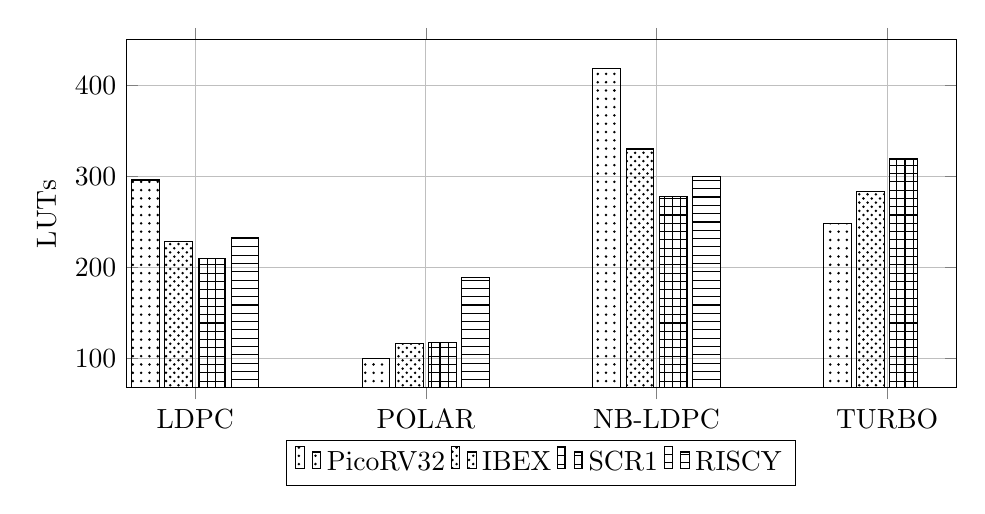
\begin{tikzpicture}
  \begin{axis}[
      width=\linewidth,
      height=6cm,
      ybar,
      %enlargelimits=0.15,
      legend style={
          at={(0.5,-0.15)},
          anchor=north,legend columns=-1
      },
      ylabel={LUTs}, 
      grid=both,
      symbolic x coords={LDPC, POLAR, NB-LDPC, TURBO},
      xtick=data,
      ]
      \addplot [pattern= dots] coordinates {(LDPC,296) (POLAR,100) (NB-LDPC,418) (TURBO,248)};
      \addplot [pattern=crosshatch dots ]coordinates {(LDPC,229) (POLAR,117) (NB-LDPC,330) (TURBO,283)};
      \addplot [pattern=grid ]coordinates {(LDPC,210) (POLAR,118) (NB-LDPC,278) (TURBO,319)};
      \addplot [pattern= horizontal lines,]coordinates {(LDPC,233) (POLAR,189) (NB-LDPC,300) };
      \legend{PicoRV32,IBEX,SCR1,RISCY};
      \end{axis}
  \end{tikzpicture}



\end{document}